\documentclass[titlepage]{article}
\usepackage[pdftex]{graphicx}

% Title
\title{Lab 4: Capacitors}
\author{Yacin Nadji}
\date{\today}

\begin{document}
\maketitle

\section{Statement of Objective}\label{sec:obj}
The purpose of this lab was to compare the values of measure effective capacitance and calculated effective capacitances in series and parallel connection, and to measure the time constant of various RC circuits. It was also meant to teach us to use the different types of equipment the lab has to offer, such as a capcimeter and a breadboard.

\section{Theory}\label{sec:theory}
\subsection{Part A: Capacitors in Series and Parallel}\label{sub:part_a-theory}
A capacitor is a device that stores charge. A very general type of capacitor is created using two conducting surfaces (sheet), separated by an insulating dielectric. The charge on the capacitor can be found using:
\begin{equation}
	Q = CV
\end{equation}
The capacitance for $n$ capacitors in series and parallel can be represented using the following equations respectively:
\begin{equation}
	\frac{1}{C} = \sum_{i = 1}^n \frac{1}{C_i}
\end{equation}
\begin{equation}
	C = \sum_{i = 1}^n C_i
\end{equation}
When a circuit is completed (generally done by closing a switch), if there is a capacitor present, charge will build up on the capacitor over a period of time. The potential across a capacitor in an RC circuit is dependent on a time constant $\tau$. This constant can be defined as:
\begin{equation}
	\tau = RC
\end{equation}

\subsection{Part B \& C: Measurement of a Time Constant}\label{sub:part_b_c_measurement_of_a_time_constant}
After the charge has been built up in a capacitor, if it is no longer being supplied a charge, the charge in the capacitor will slowly dissipate. The decay of the charge can be determined using the equation:
\begin{equation}
	ln V(t) = ln V_0 - \frac{t}{\tau}
\end{equation}
By using this equation, and measure the current charge, one can discover what the time constant, $\tau$ is. For the charging process, $\tau$ is equal to the time for $V(t)$ to reach $63\%$ of its value. For the discharging process, $\tau$ is equal to the time it takes for $V(t)$ to fall to $37\%$ of its initial value.

\section{Equipment List}\label{sec:equipment_list}
\begin{itemize}
\item[*] Capacimeter
\item[*] Set of Capacitors
\item[*] Breadboard
\item[*] Set of Resistors
\item[*] DC Power Supply
\item[*] Micronta Multimeter
\item[*] Timer
\item[*] Oscilloscope
\end{itemize}

\section{Procedure}\label{sec:procedure}
\subsection{Part A: Capacitors in Series and Parallel}\label{sub:part_a_capacitors_in_series_and_parallel-proc}
The capacitance of three capacitors were measured. They were arranged in series and parallel, and the equivalent capacitance was measured, and compared to the theoretical value.

\subsection{Part B: Measurement of a Long Time Constant}\label{sub:part_b_measurement_of_a_long_time_constant-proc}
The capacitance of a capacitor is measure. The circuit in Figure 3 of the Lab Manual is constructed. The voltmeter was set to $5 V$. The capacitor was charged. Once the capacitor was charged, the switch was opened and timing began when the voltmeter read $5 V$. The times for each half voltage were then recorded, all the way down to $0.5 V$.

\subsection{Part C: Measurement of a Short Time Constant}\label{sub:part_c_measurement_of_a_short_time_constant-proc}
The capacitance of a capacitor and resistance of a resistor were found and 
recorded.  A circuit was set up according to Figure 4 of the Lab Manual and the function 
generator was turned on and set to $250 Hz$.  Adjustments were made to the 
oscilloscope until a charging/discharging trace in Figure 4 of the Lab Manual was obtained. 
The value of t at $63\%$ of the highest voltage and at $37\%$ of the initial voltage 
was recorded as shown in Figure 2 of the Lab Manual.

\section{Data}\label{sec:data}
\subsection{Part A: Capacitors in Parallel and Series}\label{sub:part_a_capacitors_in_parallel_and_series-data}
\begin{tabular}{cc}
\hline
Capacitor & Capacitance $(nF)$\\
\hline
1 & 6.11\\
\hline
2 & 5.32\\
\hline
3 & 5.53\\
\hline
\end{tabular}\\
\\
Measured Effective Capacitance $(nF)$\\
\\
\begin{tabular}{cc}
\hline
Series & 1.894\\
\hline
Parallel & 16.9\\
\hline
\end{tabular}
\subsection{Part B: Measurement of a Long Time Constant}\label{sub:part_b_measurement_of_a_long_time_constant-data}
Discharging Capacitor\\
\begin{tabular}{cc}
\hline
V(t) & Time (s)\\
\hline
5 & 0\\
\hline
4.5 & 10.2\\
\hline
4 & 23\\
\hline
3.5 & 37.6\\
\hline
3 & 53.1\\
\hline
2.5 & 70.3\\
\hline
2 & 96.7\\
\hline
1.5 & 133.3\\
\hline
1 & 179.3\\
\hline
.5 & 267.4\\
\hline
\end{tabular}\\
\\
\begin{tabular}{cc}
\hline
Resistance of Voltmeter $(k\Omega)$ & Capacitance $(\mu F)$\\
\hline
260 & 423\\
\hline
\end{tabular}
\subsection{Part C: Measurement of a Short Time Constant}\label{sub:part_c_measurement_of_a_short_time_constant-data}
\begin{tabular}{ccc}
\hline
Charge Time to 63\% & Discharge Time to 37\% & Mean\\
\hline
$4.5 \times 10^{-4}$ & $4.0 \times 10_{-4}$ & $4.25 \times 10^{-4}$\\
\hline
\end{tabular}\\
\\
\begin{tabular}{cc}
\hline
Resistance $(k\Omega)$ & Capacitance $(nF)$\\
\hline
46 & 9.92\\
\hline
\end{tabular}

\section{Analysis of Data}\label{sec:analysis_of_data}
\subsection{Part A: Capacitors in Series and Parallel}\label{sub:part_a_capacitors_in_series_and_parallel-analysis}
For the experimental values, see \S \ref{sub:part_a_capacitors_in_parallel_and_series-data}.\\
\\
Using equations (2) and (3), the effective capacitance for $n$ capacitors in series and parallel can be calculated.\\
Series:
\[
	\frac{1}{C} = \frac{1}{6.11} + \frac{1}{5.32} + \frac{1}{5.53} = 0.532
\]
\[
	C = 1.878 nF
\]
\[
	\% Error = \frac{|1.894 - 1.878|}{1.878} * 100 = 0.8 \%
\]
\\
Parallel:
\[
	C = 6.11 + 5.32 + 5.53 = 16.9 nF
\]
\[
	\% Error = \frac{|16.9 - 16.96|}{16.96} * 100 = 0.35 \%
\]
\subsection{Part B: Measurement of a Long Time Constant}\label{sub:part_b_measurement_of_a_long_time_constant-analysis}
In order to properly use the experimental values from \S \ref{sub:part_b_measurement_of_a_long_time_constant-data}, we must change $V(t)$ into $ln V(t)$.\\
\\
\begin{tabular}{cc}
\hline
$ln V(t)$ & Time (s)\\
\hline
1.60944 & 0\\
\hline
1.50408 & 10.2\\
\hline
1.38629 & 23\\
\hline
1.25276 & 37.6\\
\hline
1.09861 & 53.1\\
\hline
0.916291 & 70.3\\
\hline
0.693147 & 96.7\\
\hline
0.405465 & 133.3\\
\hline
0.000000 & 179.3\\
\hline
-0.693147 & 267.4\\
\hline
\end{tabular}\\
If we graph this relationship, we end up with a nearly linear function, with the value for slope being $m = -\frac{1}{\tau}$.\\
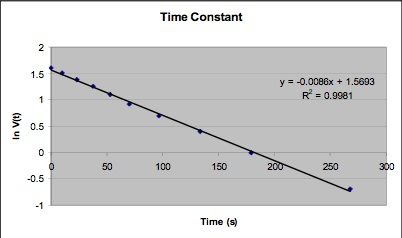
\includegraphics{1.jpg}\\
\\
In this case, $m = -0.0086s^{-1}$. Taking the negative reciprocal of $m$ gives us the time constant, $\tau$, which is $\tau = 116.279 s$. The theoretical value for $\tau$ can be calculated using equation (4):
\[
	\tau = 284000 \Omega \times 0.000423 F = 109.98s
\]
\[
	\% Error = \frac{|116.279 - 109.98|}{109.98} * 100 = 5.72 \%
\]
\subsection{Part C: Measurement of a Short Time Constant}\label{sub:part_c_measurement_of_a_short_time_constant-analysis}
The time constant, $\tau$, calculated by the product of $RC$ obtained from the values of $R$ and $C$ in \S \ref{sub:part_c_measurement_of_a_short_time_constant-data} is $0.0456 ms$. The experimental value is $0.0425$.
\[
	\% Error = \frac{|0.0456 - 0.0425|}{0.0425} * 100 = 7.29 \%
\]

\section{Discussion of Results}\label{sec:discussion_of_results}
\subsection{Part A: Capacitors in Series and in Parallel}\label{sub:part_a_capacitors_in_series_and_in_parallel-results}
In Part A, the values were quite close. For the series connection we landed a very positive \% error of $0.8 \%$. The \% error for the expected capacitance was another great value of $0.35 \%$. The only possible cause for error could be a small machine error between measuring, and the actual values of the capacitors.

\subsection{Part B: Measurement of a Long Time Constant}\label{sub:part_b_measurement_of_a_long_time_constant-results}
In Part B, the values didn't turn out as well. The \% error for Part B was $5.4 \%$. The possible source of this error is most likely a human one, due to the fact that we were measuring the time by hand, so it was entirely possible to make errors.

\subsection{Part C: Measurement of a Short Time Constant}\label{sub:part_c_measurement_of_a_short_time_constant-results}
In Part C, we had similar results as in Part B. We had a \% error of $6.8 \%$. This error is probably a result of an error in how we calibrated the oscilloscope.

\section{Conclusions}\label{sec:conclusions}
The results in Part A reinforce the relationship between the effective 
capacitance and the individual capacitances in the way which equation (2) 
and (3) state. In part B and C, the results, and the linearity of Graph 1, 
indicate that the time constant of $RC$ circuit is, indeed, the product of $R$ and 
$C$.

\end{document}